\documentclass[a4paper]{article}

%% Language and font encodings
\usepackage[english]{babel}
\usepackage[utf8x]{inputenc}
\usepackage[T1]{fontenc}

%% Sets page size and margins
\usepackage[a4paper,top=3cm,bottom=2cm,left=2cm,right=2cm,marginparwidth=1.75cm]{geometry}

%% Useful packages
\usepackage{amsmath}
\usepackage{graphicx}
\setlength{\marginparwidth}{2cm}
\usepackage[colorinlistoftodos]{todonotes}
\usepackage[colorlinks=true, allcolors=blue]{hyperref}

\title{anthro-c12ac}
\author{Myles Fung}
\date{Fall '22}

\begin{document}

\begin{figure}
\centering
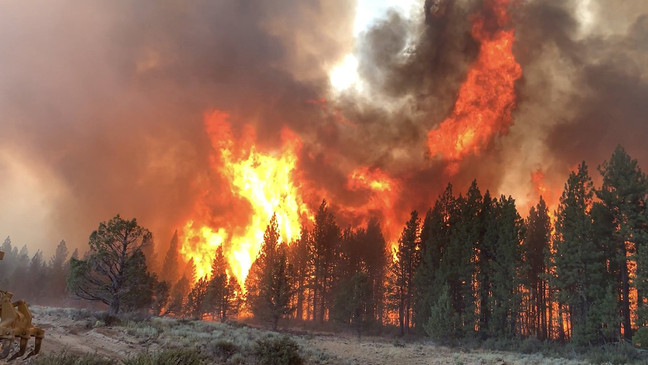
\includegraphics[width=.5\textwidth]{conflagration.jpeg}
\caption{\label{fig:conflagration}A conflagration.}
\end{figure}

\maketitle


\section{Week 1, 8/22}

\subsection{}


\section{Week 2, 8/29: <chapter title>}

\subsection{<topic>}
Fire ecology 

\begin{itemize}
    \item item 1
    \item item 2
\end{itemize}

Fire ecology



\subsection{<topic 2>}

\begin{itemize}
    \item item 1
    \item item 2
\end{itemize}


\section{Chapter 2: <chapter title>}

\subsection{<topic>}
Fire ecology \dots 


\end{document}